% arara: pdflatex
%        File: ComplexAnalysis.tex
%     Created: Sat Jun 24 03:00 PM 2023 B
% Last Change: Sat Jun 24 03:00 PM 2023 B
%
\documentclass[a4paper, 12pt]{article}
\usepackage[]{amsmath}
\usepackage{amsthm}
\usepackage{amssymb}
\usepackage{mathtools}
\usepackage{soul}
\usepackage[]{graphicx}
\graphicspath{ {./images/} }
\usepackage{caption}
\usepackage{subcaption}

\theoremstyle{definition}
\newtheorem{definition}{Definition}
\newtheorem{exercise}{Exercise}
\newtheorem{example}{Example}
\newtheorem{remark}{Remark}

\numberwithin{definition}{section}
\numberwithin{exercise}{section}
\numberwithin{remark}{section}
\numberwithin{figure}{section}
\numberwithin{example}{section}

\newcommand{\R}{\mathbb{R}}
\newcommand{\C}{\mathbb{C}}

\title{Complex Analysis Summary}
\author{Paul Joo-Hyun Kim}
\begin{document}
\maketitle
\setcounter{section}{-1}
\section{Preface}
This note is for people studying complex analysis,
and got lost in the middle with bunch of technical explanations.
I wil try my best to be succinct as possible,
stating important results (mostly without proof, but a bit of justification).

\textbf{Warning}: This summary note is not a substitute for the lecture note.
Make sure you study from lecture note!

\section{Complex Plane and M\"obius Maps}
\subsection{Complex Plane and Complex Infinity}
We will be working in what's known as the \textit{extended complex plane}.
Define the symbol $\C_{\infty} \coloneqq \C \cup \left\{ \underbrace{\infty}_{\text{Complex Infinity}} \right\}$;
that is, I refer to the space of complex numbers
and infinity.

Note that in $\C_{\infty}$, $\infty$ is different from infinity in real numbers.
$\infty \coloneqq \frac{1}{0}$ is a value that is not ``larger'' or ``smaller'' than any number
(since we are talking about complex number\dots), but rather
a number on a complex plane at a really far distance from origin.

It is \textbf{WRONG} to say:
\begin{itemize}
    \item $\infty \geq a$ for any $a \in \C_{\infty}$
    \item $\infty \leq a$ for any $a \in \C_{\infty}$
\end{itemize}
However, it is \textbf{CORRECT}\footnote{
    Subtlety here: it seems a bit dodgy to say $\infty = \infty_{\infty}$,
    but this is matter of definition;
    you won't really encounter this type of ``philosophical'' problem
    in your exam.
} to say:
\begin{itemize}
    \item $|\infty| \geq |a|$ for any $a \in \C_{\infty}$.
\end{itemize}
$\infty$ is not like a point on $\C$, but rather like a gigantic circle that you can never reach.

\subsection{M\"obius Maps}
\begin{definition}[M\"obius Map]
    $\psi : \C_{\infty} \rightarrow \C_{\infty}$ is a \textbf{M\"obius map} if:
    \begin{equation*}
        \psi \left( z \right) \coloneqq \frac{az + b}{cz + d}
    \end{equation*}
    where $
    \begin{pmatrix}
        a & b \\ c & d
    \end{pmatrix}
    $ is a nonsingular matrix.
    (This restriction removes the possibility of $\frac{0}{0}$,
    or trivial maps (eg: Constant function).)

    One needs to be careful when defining this function at infinity,
    but it should be sensible.\footnote{
    That said, if you are supposed to define what a M\"obius map is,
    you are \textbf{required} to definitions involving infinity as well.
    }
\end{definition}
\begin{exercise}[Composition of two M\"obius map is a M\"obius map]
    Show that for two M\"obius maps $\psi_1, \psi_2$,
    its composition $\psi_1 \circ \psi_2$ is also a M\"obius map.
\end{exercise}
\begin{remark}
    Consider the $2 \times 2$-matrix-to-M\"obius-map map as follows:
    \begin{equation*}
        f (A) \coloneqq
        \begin{pmatrix}
            a_{11} & a_{12} \\ a_{21} & a_{22}
        \end{pmatrix}
        \mapsto
        \frac{a_{11} z + a_{12}}{a_{21} z + a_{22}}
    \end{equation*}
    Then it turns out that
    $f\left( AB \right) = f(A) f(B)$
\end{remark}
\begin{exercise}[Decomposition of M\"obius maps]
    It turns out that M\"obius maps can be written as composition of
    \begin{itemize}
        \item translation
        \item dialation (``scaling by nonzero constant'')
        \item inversion ($z \mapsto \frac{1}{z}$)
    \end{itemize}
    Prove this. (Hint: You can do a constructive proof.)
\end{exercise}
M\"obius maps also has a very convenient property:
\begin{exercise}[Circline to Circline]
    Show that M\"obius maps map circlines to circline.
    (This means a line will either map to a circle or a line,
    and also a circle will either map to a circle or a line.)

    (Note: This is a boring long tedious proof, that probably won't be asked in exam,
    but don't take my word for it.)
\end{exercise}

\section{Complex Differentiability}
Complex differentiability is one of the highlights of the complex analysis.
\begin{definition}[Differentiable Function AKA Holomorphic Function]
    Take $a \in \C$.
    Let $f:U \rightarrow \C$ be a function where $U$ is a neighbourhood\footnote{Some open set containing $a$.} of $a$.
    Then $f$ is \textbf{(complex) differentiable} or \textbf{holomorphic} at $a$ if
    \begin{equation*}
        f'(a) = \lim_{z \rightarrow a} \frac{f(z) - f(a)}{z - a}
    \end{equation*}
    exists, and call it derivative of $f$ at $a$.
    If $f$ is differentiable for all points in $U$, then it is said to be
    differentiable/holomorphic on $U$.
\end{definition}
\begin{remark}
    Note that the definition seems to be have trivially extended from real analysis.
    \ul{However, there is a subtlety}.
    The limit does not approach just from positive or negative side,
    but from any direction. (Figure \ref{fig: Real and Complex Limit})
    \begin{figure}[tbp]
        \centering
        \begin{subfigure}[b]{0.5\textwidth}
            \centering
            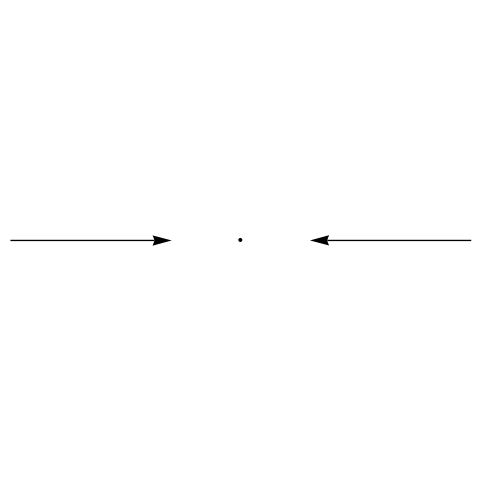
\includegraphics[width=\textwidth]{realLimit}
            \caption{Real Limit}
        \end{subfigure}
        \hfill
        \begin{subfigure}[b]{0.5\textwidth}
            \centering
            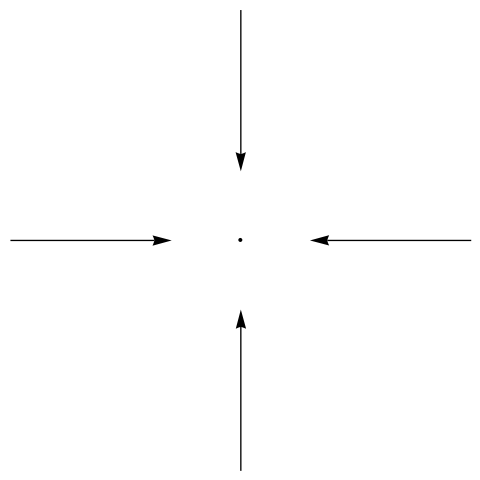
\includegraphics[width=\textwidth]{complexLimit}
            \caption{Complex Limit}
        \end{subfigure}
        \caption{Real limit (former) only concerns the approaching value from left and right side, but complex limit (latter) oncerns the approaching value from all direction.}
        \label{fig: Real and Complex Limit}
    \end{figure}
\end{remark}
\begin{exercise}[Differentiation Rules]
    Show that all differentiation rules from real analysis holds
    with holomorphic functions.
    \begin{itemize}
        \item Sum
        \item Product Rule
        \item Quotient Rule
        \item Chain Rule
    \end{itemize}
\end{exercise}
Due to the definition of complex limits being more restrictive,
a more nontrivial result follows.
\begin{exercise}[Cauchy-Riemann Equations]
    Let $a \in \C$ and $U$ be a neighbourhood of $a$.
    $f : U \rightarrow \C$ be holomorphic $a$.
    Write $f(z) = u(x,y) + i v(x,y)$ where $u,v$ are real functions
    and $z = x + iy$ where $x,y \in \R$.
    Then $\partial_x u, \partial_y u, \partial_x v, \partial_y v$ all exist,
    and the following \textbf{Cauchy-Riemann equations} hold:
    \begin{align*}
        \partial_x u &= \partial_y v \\
        \partial_x v &= - \partial_y u
    \end{align*}
(Hint: Figure \ref{fig: Real and Complex Limit} might give you an insight.)
\end{exercise}
\begin{remark}
    If Cauchy-Riemann does not hold, then it must mean that $f$ is not holomorphic! (Consider $f(z) = \bar{z}$. Cauchy-Riemann does not hold for any point, so it is nowhere holomorphic.)
\end{remark}
\begin{exercise}
    If $f(z) = u(x,y) + i v(x,y)$ is holomorphic on $U$,
    and $u,v$ are twice differentiable,
    deduce that $u$ and $v$ are \textit{harmonic}, that is,
    they satisfy the Laplace equation $\Delta u = \Delta v = 0$.
\end{exercise}
\begin{remark}
    It turns out complex plane reveals a lot about solving Laplace equation!
\end{remark}
Here is another kicker:
\begin{exercise}[Cauchy-Riemann to Holomorphic]
    If the partial derivatives exist and are continuously differentiable,
    Cauchy-Riemann implies holomorphicity.
\end{exercise}
\begin{remark}
    This means if you check that Cauchy-Riemann holds, you can immediately assume you can construct an analytic function!
\end{remark}
Holomorphic functions also have Taylor expansion:
\begin{remark}[Holomorphic functions have Taylor expansion]
    If $f$ is holormorphic at $a$, then
    in a neighbourhood of $a$, you can write
    \begin{equation*}
        f(z) = \sum_{n=0}^{\infty} c_n \left( z-a \right)^n
    \end{equation*}
    All the formulae for Taylor expansion holds (term-by-term differentiation, etc.)
\end{remark}
\begin{example}[Common Function Definitions]
    Here are definitions for some of the functions.
    \begin{align*}
        e^z = \exp z &\coloneqq \sum_{n=0}^{\infty} \frac{z^n}{n!} \\
        \cos{z} &\coloneqq \sum_{n=0}^{\infty} \left( -1 \right)^n \frac{z^{2n}}{\left( 2n \right)!} \\
        \cos{z} &\coloneqq \sum_{n=0}^{\infty} \left( -1 \right)^n \frac{z^{2n+1}}{\left( 2n + 1\right)!}
    \end{align*}
\end{example}
\begin{exercise}
    Show that
    \begin{align*}
        \cos{z} &= \frac{e^{iz} + e^{-iz}}{2} \\
        \sin{z} &= \frac{e^{iz} - e^{-iz}}{2i}
    \end{align*}
\end{exercise}
\begin{exercise}
    Show that $\exp \left( z+w \right) = \exp (z) \exp (w)$
\end{exercise}
\section{Branch Cut}
Sometimes, there is just no sensible way to define a function that it is holomorphic everywhere\dots
One of the unfortunate (or fortunate) functions is the logarithm.
\begin{example}
    Define logarithm function as:
    \begin{equation*}
        \log z \coloneqq \log |z| + i \theta
    \end{equation*}
    where $\theta$ is the argument of $z$.

    The choice of the interval for $\theta$ changes the behaviour of $\log z$ function.
    For example, one could take the interval to be $\left[ 0, 2\pi \right)$,
    or one could take it to be $\left[ - \pi, \pi \right)$,
    or even just $\left[a, a + 2\pi\right)$.
\end{example}
\end{document}


